%% LaTeX2e class for student theses
%% sections/apendix.tex
%% 
%% Karlsruhe Institute of Technology
%% Institute of Information Security and Dependability
%% Software Design and Quality (SDQ)
%%
%% Dr.-Ing. Erik Burger
%% burger@kit.edu
%%
%% Version 1.6, 2024-06-07

\iflanguage{english}
{\chapter{Appendix}}    % english style
{\chapter{Anhang}}      % german style
\label{chap:appendix}


%% -------------------
%% | Example content |
%% -------------------
\section{First Appendix Section}
\label{sec:appendix:FirstSection}
		
\setcounter{figure}{0}


\begin{figure}[ht]
    \centering
    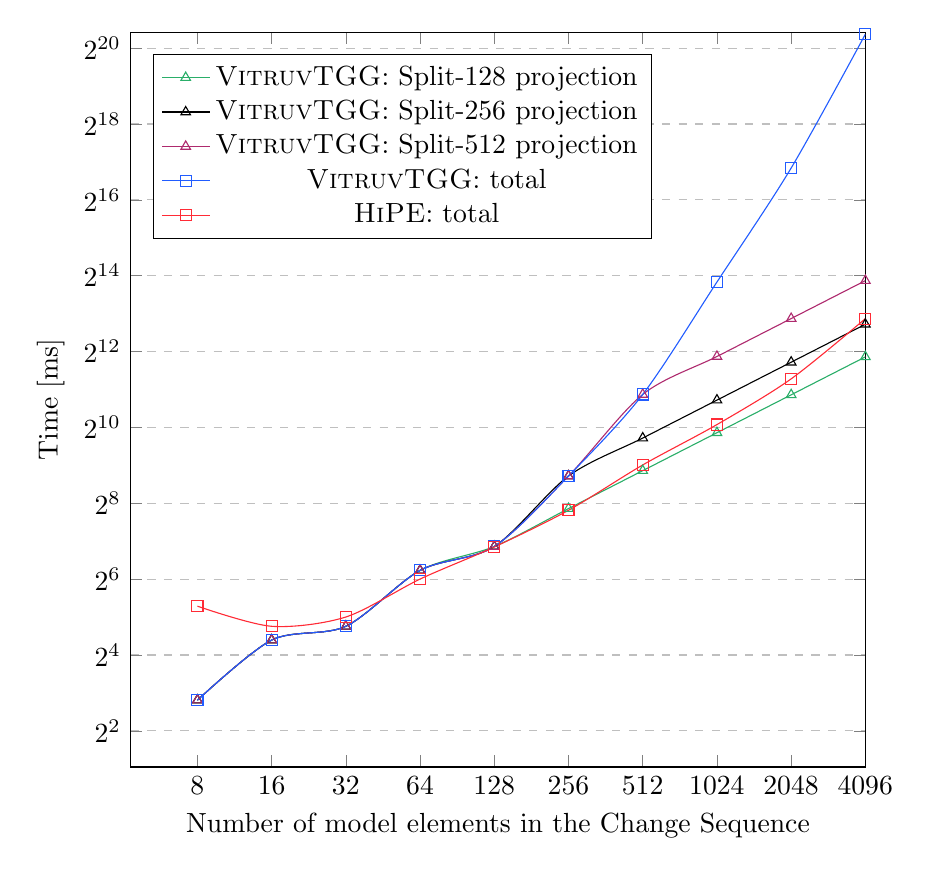
\begin{tikzpicture}
        \definecolor{myBlue}{RGB}{33,92,255}
        \definecolor{myRed}{RGB}{255,43,54}
        \definecolor{myGreen}{RGB}{42,174,105}
        \definecolor{myPurple}{RGB}{174,42,110}
        \begin{axis}[
            width=0.9\textwidth,
            height=0.9\textwidth,
            xlabel={Number of model elements in the Change Sequence},
            ylabel={Time [ms]},
            xmin=0, xmax=4096,
            ymin=0, ymax=1400000,
            xticklabels={4,8,16,32,64,128,256,512,1024,2048,4096},
            % ytick={0,10,100,1000,10000,100000},
            legend pos=north west,
            ymajorgrids=true,
            grid style=dashed,
            xmode=log,
            ymode=log,
            log basis x={2},
            log basis y={2}
        ]
        
        % VitruvTGG Split-128:
        \addplot[
            color=myGreen,
            mark=triangle,
            smooth,
            % opacity=0.4,
            ]
            coordinates {
            % (8,0)(16,6)(32,4)(64,9)(128,12)(256,45)(512,145)(1024,564)(2048,2191)
            (8,7)(16,21)(32,27)(64,75)(128,116)(256,232)(512,464)(1024,928)(2048,1856)(4096,3712)
            };
        % VitruvTGG Split-256:
        \addplot[
            color=black,
            mark=triangle,
            smooth,
            % opacity=0.4,
            ]
            coordinates {
            % (8,0)(16,3)(32,2)(64,4)(128,2)(256,7)(512,24)(1024,88)(2048,273)
            (8,7)(16,21)(32,27)(64,75)(128,116)(256,421)(512,842)(1024,1684)(2048,3368)(4096,6736)
            };
        % VitruvTGG Split-512:
        \addplot[
            color=myPurple,
            mark=triangle,
            smooth,
            % opacity=0.4,
            ]
            coordinates {
            % (8,0)(16,2)(32,2)(64,9)(128,42)(256,189)(512,1123)(1024,8241)(2048,96266)
            (8,7)(16,21)(32,27)(64,75)(128,116)(256,421)(512,1869)(1024,3738)(2048,7476)(4096,14952)
            };
        % VitruvTGG TOTAL:
        \addplot[
            color=myBlue,
            mark=square,
            smooth,
            ]
            coordinates {
            % (8,4)(16,25)(32,22)(64,55)(128,112)(256,386)(512,1728)(1024,10625)(2048,103277)
            (8,7)(16,21)(32,27)(64,75)(128,116)(256,421)(512,1869)(1024,14577)(2048,117092)(4096,1350937)
            };
        % HIPE TOTAL:
        \addplot[
            color=myRed,
            mark=square,
            smooth,
            ]
            coordinates {
            % (8,48)(16,18)(32,35)(64,56)(128,114)(256,209)(512,436)(1024,1138)(2048,2297)
            (8,39)(16,27)(32,32)(64,64)(128,115)(256,225)(512,515)(1024,1077)(2048,2484)(4096,7467)
            };
        \legend{
            \textsc{VitruvTGG}: Split-128 projection,
            \textsc{VitruvTGG}: Split-256 projection,
            \textsc{VitruvTGG}: Split-512 projection,
            \textsc{VitruvTGG}: total, 
            \textsc{HiPE}: total
        }
            
        \end{axis}
    \end{tikzpicture}
    \caption[Runtime complexity projection trend of\textsc{VitruvTGG} with split change sequence]{Runtime complexity projection trend of \textsc{VitruvTGG} with split change sequence and \textsc{HiPE}, different split sizes.}
    \label{fig:eval:RuntimeTrendSplitProjection}
\end{figure}
